\chapter{Aufbau des Prüfstands und Grundlagen}
\section{Grundlagen des Prüfstandes}
In diesem Kapitel wird der verwendete Schaltaktorikprüfstand des IMS vorgestellt, an dem  die Entwicklung des Smart Actuators stattgefunden hat. Beschrieben wird der Aufbau des Prüfstands, wie er vor den Änderungen im Rahmen dieses Projektes vorlag. Die Konstruktion des Prüfstandes erfolgte in vorangegangenen Arbeiten und wurde seitdem stetig weiterentwickelt. An ihm werden Schaltaktoriksysteme für Fahrzeugantriebe untersucht. Abbildung \ref{fig:Pruefstand} zeigt die in dieser Arbeit verwendeten Subsysteme des Prüfstandes. Im Folgenden erfolgt zunächst die Vorstellung des mechanischen Aufbaus, woraufhin der elektronische Aufbau anschließt. 
\begin{figure}[h]
	\centering
		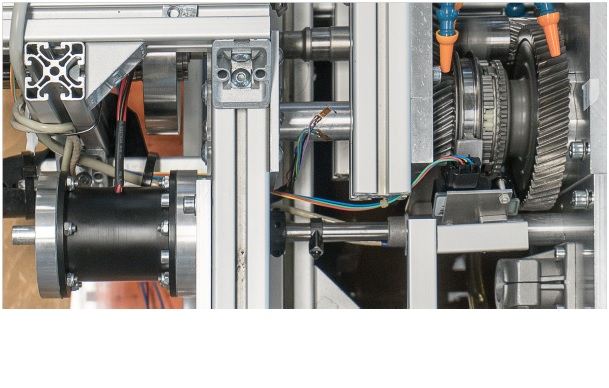
\includegraphics{Bilder/Pruefstand.jpg}
	\caption{Prüfstand \cite[S.5]{adp}}
	\label{fig:Pruefstand}
\end{figure}
\subsection{Getriebe allgemein}

Ein Getriebe ist im Automobil dafür zuständig, die Drehzahl des Motors in ein Drehmoment umzuwandeln, welches die Räder antreibt. Da Motoren nur einen kleinen Bereich von Motordrehzahlen abdecken werden mehrstufige Getriebe verwendet, die verschiedene Raddrehzahlen durch unterschiedliche Übersetzungsverhältnisse bereitstellen können.  Das Einstellen des jeweiligen Ganges kann dabei per Hand (Handschaltgetriebe) oder automatisiert über einen Aktor (Schaltaktorik) erfolgen. 
Im Fahrzeuggetriebe, beispielhaft dargestellt in \ref{fig:Fahrzeuggetriebe} ist die Eingangswelle, welche durch den Motor angetrieben wird, über eine Zahnradverbindung  fest mit der  Vorgelegewelle verbunden. Auf ihr sind noch weitere fest fixierte Zahnräder angebracht, deren Anzahl mit den verfügbaren Gängen übereinstimmt. Diese greifen jeweils in Losräder auf der Abtriebswelle. Um einen bestimmten Gang einzulegen muss nun das jeweilige Losrad für den Moment fest mit der Abtriebswelle verbunden werden, sodass nur diese Zahnverbindung ein Drehmoment überträgt. Dies geschieht über eine formschlüssige Verbindung mit einer Schaltmuffe, die über die durch den Aktor angetrieben Schaltgabel in Position gebracht wird.

\begin{figure}[h]
	\centering
		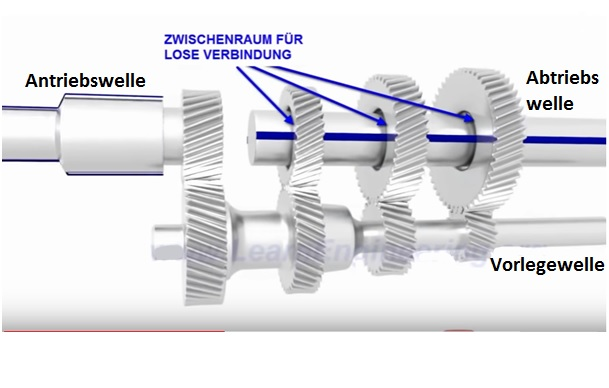
\includegraphics{Bilder/Fahrzeuggetriebe.jpg}
	\caption{Fahrzeuggetriebe}
	\label{fig:Fahrzeuggetriebe}
\end{figure}

\subsection{Getriebe des Prüfstands}

Der Prüfstand besitzt zwei Gänge, in die über eine Schaltgabel geschaltet werden kann. Eine Bewegung der Schaltgabel nach links legt Gang 1 über eine mechanische Synchronisierung ein, während mit Hilfe einer Bewegung nach rechts die Schaltung des Ganges 2 durch eine Klauenkupplung erfolgt. Somit können sowohl Schaltaktoriksysteme mit als auch ohne Synchronring untersucht werden.
Die Bewegung der Schaltgabel wird durch einen Linearaktor ermöglicht, welcher von außen an das Item-Profil verschraubt ist. In diesem ist eine Tauchspule verbaut, die die benötigten Kräfte auf die Läuferstange aufbringt. Über eine starre Wellenkupplung sind Läuferstange und Schaltgabel miteinander verbunden, wodurch die Kräfte auf die Schaltgabel übertragen werden und Schaltvorgänge ermöglicht werden.

\subsection{Aktor}

Der momentan in dem Prüfstand verbaute Tauchspulenaktor wurde von Oliver Hahn im Rahmen seiner Bachelorthesis entwickelt und konstruiert. Er übernimmt im automatisierten Schaltvorgang die Aufgabe, die Schaltgabel  über die Schaltstange translatorisch zu verschieben, welche ursprünglich mit einem Schalthebel per Hand ausgeführt wurde. Die Übertragung des Schaltbefehls an den Getriebeaktor erfolgt dabei durch ein elektrisches Signal (\textit{shift by wire})
Sein Querschnitt ist in folgender Abbildung schematisch dargestellt.

\begin{figure}[h]
	\centering
		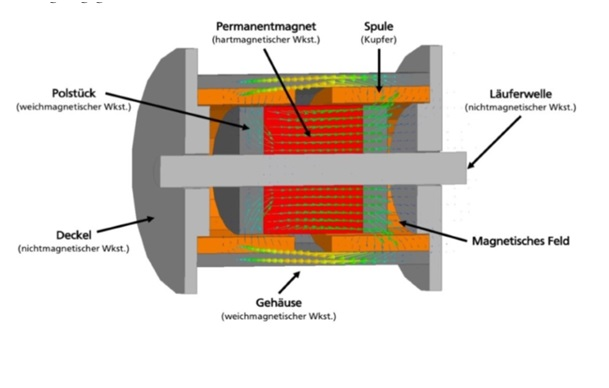
\includegraphics{Bilder/Querschnitt Aktor.jpg}
	\caption{Querschnitt Tauchspulenaktor \cite[S.30]{Hahn2018}}
	\label{fig:Querschnitt Aktor}
\end{figure}

Sein Aufbau ist zylindrisch und kann in den ortsfesten Stator und den beweglichen Läufer unterteilt werden. Der Stator des Aktors besteht aus zwei in Reihe geschalteten Kupferspulen, welche fest in dem Gehäuse aus Weicheisen liegen und nach oben und unten mit Deckeln aus Aluminium fixiert werden. Der Läufer besteht aus einer nichtmagnetischen Läuferwelle, auf der sich fünf Permanentmagneten aus Neodym-Eisen-Bor befinden, welche mit Hilfe von zwei Polstücken aus Weicheisen axial auf der Läuferstange montiert sind. 
Werden nun die Kupferspulen von Strom durchflossen, so wirkt eine vom Magnetfeld der Permanentmagneten induzierte Lorentzkraft orthogonal auf sie. Diese Kraft ist abhängig von der Stromstärke I, der magnetischen Flussdichte der Permanentmagneten B und der vom Magnetfeld durchsetzten Leiterlänge l:
	\[F=I*l*B
\]
Da die Spulen jedoch fest im Gehäuse verbaut sind, wirkt eine entgegengerichtete Kraft auf die Permanentmagneten, die auf der axial verschiebbaren Läuferwelle lagern. Diese Kraft bewirkt dann eine translatorische Bewegung der Welle und somit auch der Schaltgabel. Die Richtung der translatorischen Bewegung kann dabei über die Richtung des in den Spulen fließenden Stromes, der Betrag der Kraft über den Betrag des Stromes eingestellt werden.
Anhand von Abbildung \ref{fig:Kennlinie Aktor} ist zu erkennen, dass die Kraft-Weg Kennlinien des Aktor innerhalb des Nutzungsbereichs von -10 Millimeter bis +10 Millimeter bei verschiedenen Stromstärken annähernd linear verlaufen. 

\begin{figure}[h]
	\centering
		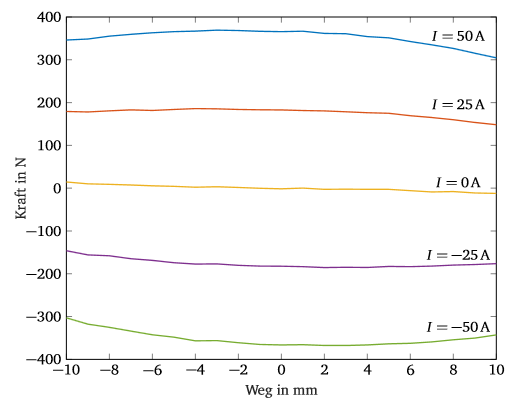
\includegraphics{Bilder/Kennlinie Aktor.png}
	\caption{Kraft-Weg-Strom Kennlinien des Tauchspulenaktors \cite[S.12]{adp}}
	\label{fig:Kennlinie Aktor}
\end{figure}

\subsection{Aktoransteuerung}

Zur Aktoransteuerung wird ein Arduino IBT2 Motortreiber verwendet, die Stromversorgung erfolgt über ein Manson SBC-2130 Battery Charger im Power Supply Mode. Der Motortreiber besteht aus zwei BTS7960 MOSFETs, die je nach Vorgabe des pulsdauermodulierten Signals (PWM-Frequenz) eine Spannung von bis zu 13,8V an den Aktor durchschalten. 

\subsection{Autobox}

\subsection {Positionsmessung und -regelung}

Die Position der Läuferstange wird über einen PLCD-25M Sensor gemessen, dessen berührungslose PLCD (permanentmagnetic linear contactless displacement) Technologie die magnetische Sättigung nutzt. Der weichmagnetische Kern des Sensors ist über seine komplette Länge von einer Primärspule umgeben. Auf der Schaltgabel ist ein Permanentmagnet befestigt, welcher je nach Position zu einer lokalen Sättigung des weichmagnetischen Kerns führt. Über zwei Auswertungsspulen am Rand des Sensors kann nun die Position der Sättigungszone entlang der Sensorachse über eine induzierte Spannung bestimmt werden.

\begin{figure}[h]
	\centering
		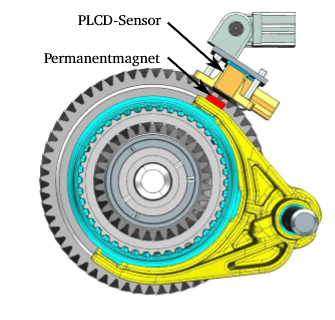
\includegraphics{Bilder/Sensor.png}
	\caption{Einbauposition PLCD Sensor an der Schaltgabel \cite[S.14]{adp}}
	\label{fig:Sensor}
\end{figure}
Der Sensor wird an die MicroAutoBox zwecks Spannungsversorgung sowie zur Durchführung der Kalibrierung angeschlossen. Die Kalibrierung wurde in (Quelle) entwickelt und erfolgt bisher bei jedem Start. 

Die bisherige Regelung der Schaltgabelposition wurde in einem vorherigen Advanced Design Project ausgelegt. Dazu wurden mithilfe des Ziegler-Nichols-Verfahren zunächst Parameter für einen PID-Regler ermittelt, welcher allerdings noch zu große Totzeiten und ein Überschwingen aufwies. In einer anschließenden iterativen Optimierung mit Störgrößenkompensation wurden die Regelparameter zu KP =2,6\%V/mm, KI =20\%V/smm und KD =1,6\%Vs/mm bestimmt. Der Verlauf der Sprungantwort ist in nachstehender Abbildung (\ref{fig:Sprungantwort Schaltgabelposition}) dargestellt.
\begin{figure}[h]
	\centering
		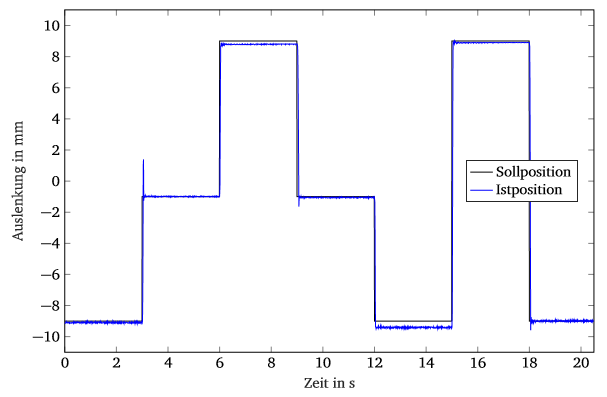
\includegraphics{Bilder/Sprungantwort Schaltgabelposition.png}
	\caption{Sprungantwort Schaltgabelposition \cite[S.35]{adp}}
	\label{fig:Sprungantwort Schaltgabelposition}
\end{figure}

\section{Grundlagen Löten}
Löten gehört zu den Fügeverfahren und bezeichnet das Verbinden zweier Metalle durch eine Metalllegierung unter Einfluss von Wärme \cite{löten}. Die Metalllegierung wird dabei als Lot bezeichnet und hat eine geringere Schmelztemperatur (Liquidustemperatur) als die beiden zu verbindenden Metalle (Solidustemperatur). Durch das Löten entsteht eine feste, korrosionsbeständige sowie strom- und wärmeleitende Verbindung. Lötverfahren werden nach Arbeitstemperatur eingeteilt: es wird unterschieden in Weichlöten (bis 450°C), Hartlöten (450°C - 900°C) und Hochtemperaturlöten (über 900°C). Im Rahmen dieses Projektes wurde das Verfahren Weichlöten mit Lötkolben angewendet, um die elektrischen Bauteile auf der Platine anzubringen. Dazu konnten die vom Institut bereitgestellten Lötstationen und –materialien verwendet werden. 

\section{Mikrocontroller}
Ein Mikrocontroller (\textit{MCU: microcontroller unit}) ist ein hochintegrierter Halbleiterchip, der ein komplettes Mikrorechnersystem enthält. Prozessoren, Speicher, Ein- und Ausgabegeräte sind somit auf einem kleinen Chip enthalten der zum Ziel hat, Steuerungs- und Kommunikationsaufgaben möglichst simpel mit wenig Bauelementen zu bearbeiten. 
\begin{figure}[h]
	\centering
		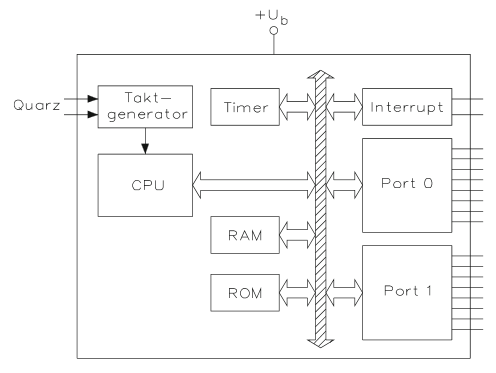
\includegraphics{Bilder/Blockschaltbild Mikrocontroller.png}
	\caption{Blockschaltbild eines typischen Mikrocontrollers \cite[S.3]{Bernstein2015}}
	\label{fig:Blockschaltbild Mikrocontroller}
\end{figure}

In Abbildung \ref{fig:Blockschaltbild Mikrocontroller} ist der typische Aufbau eines Mikrocontroller dargestellt. Die Schnittstellen zur Peripherie sind durch einen Betriebsspannungsanschluss, einen Takteingang, an den in der Regel ein Quarz angeschlossen wird, sowie die Portleitungen  gegeben. Bei den Ports wird zwischen Eingangskanälen (\textit{\textbf{I}nput Port}), die digitale Signale lesen, und Ausgangskanälen (\textit{\textbf{O}utput Port}, die digitale Signale setzen beziehungsweise löschen, unterschieden. Des weiteren können I/O Pins digital oder analog sein, wobei analoge Signale mithilfe eines Analog/Digital Wandlers (AD-Wandler) zuerst in digital Signale umgewandelt werden müssen, damit der Mikrocontroller sie verarbeiten kann.
Eine Spezialform von Eingängskanälen sind die Interrupt-Pins, die bei bestimmten Ereignissen Unterbrechungen des laufenden Programms verursachen, um temporär einen anderen Vorgang zu bearbeiten. 

Intern sind die einzelnen Bausteine, die im folgenden kurz erläutert werden, über ein Bussystem verbunden.
Der Prozessor (\textit{CPU: central processing unit} führt Berechnungen und logische Operationen durch.
Der Taktgenerator gibt die Arbeitsfrequenz an, also wie schnell der CPU arbeiten soll.
Der Arbeitsspeicher (\textit{RAM: random access memory} speichert temporär Daten, die aber spätestens nach dem Entfernen der Betriebsspannung gelöscht werden.
Der Festspeicher (\textit{ROM: read only memory} behält seinen Speicherinhalt auch nach dem Entfernen der Betriebsspannung und enthält aufgrund dessen das Programm sowie Einstellungen und wichtige Daten. Im Vergleich zum RAM hat er eine langsame Schreibgeschwindigkeit. 
Der Timer hilft dabei, Anzahlen von Ereignissen zu zählen oder Zeitabstände zu messen, indem er Spannungswechsel an einem Eingangskanal zählt. 

Die genaue Ausführung des Chips kann je nach Aufgabentyp variieren, sodass eine Vielzahl an verschiedenen Mikrocontrollern erhältlich ist. Diese unterscheiden sich meistens in der Größe des Speichers, in der Anzahl der Anschlüsse beziehungsweise Schnittstellen, in der Bitbreite, in den Taktraten sowie in der Bauform. Typischerweise werden Mikrocontroller in eingebetteten Systemen (\textit{embedded systems} verwendet, bei denen die Steuereinheit direkt im System selbst integriert ist. Übliche Anwendungen für Mikrocontroller sind Roboter, Handys, Temperaturregler oder Motorsteuerungen \cite{Brinkschulte}. 

\subsection{Eingebettete Systeme und Smart Actuators}
Eingebettete Systeme werden definiert als Rechenmaschinen, die für den Anwender weitgehend unsichtbar in einem technischen System eingebettet sind und mit diesem in Wechselwirkung stehen \cite[S.8]{Gessler2014}. Der Rechner kann dabei für Regelungs-, Steuer- oder Überwachungsaufgaben und/ oder für Signal- und Datenverarbeitung zuständig sein. Der allgemeine Zweck ist es, die Stellglieder als Reaktion auf Eingangssignale, die von Sensoren oder manuell vorgegeben werden, zu steuern \cite[S.1]{Broy2003}. Eingebettete Systeme werden oft für speziell eine isolierte Aufgabe entwickelt und angepasst.
Ein Aktor, beziehungsweise Aktuator (aus dem englischen: \textit{actuator}) ist dafür da, die elektrischen Signale in eine Bewegung oder Kraft umzusetzen und bildet somit das Stellglied. Das Konzept des intelligenten Aktors (\textit{smart actuator}) beinhaltet neben dem Aktor selbst auch den restlichen Regelkreis, also Aktoransteuerung, Sensorik, Systemdiagnostik und die Recheneinheit \cite[S.442]{smartactuator}. Vereinfacht gesagt umfasst also ein Smart Actuator den Aktor plus die eingebettete Elektronik.
Smart Actuators reduzieren beziehungsweise ersetzen die benötigte Interaktion mit einem Menschen oder externen Rechner und können somit effektiver und schneller arbeiten. Außerdem kann oft viel Bauraum eingespart werden, es gibt weniger Komponenten und deutlich weniger Verkabelung
